\documentclass[tikz,border=4pt]{standalone}
\usepackage{tikz}
\usepackage{amsmath}
\usetikzlibrary{arrows.meta,calc,positioning,shapes.geometric,shapes.misc,backgrounds,fit}

\begin{document}
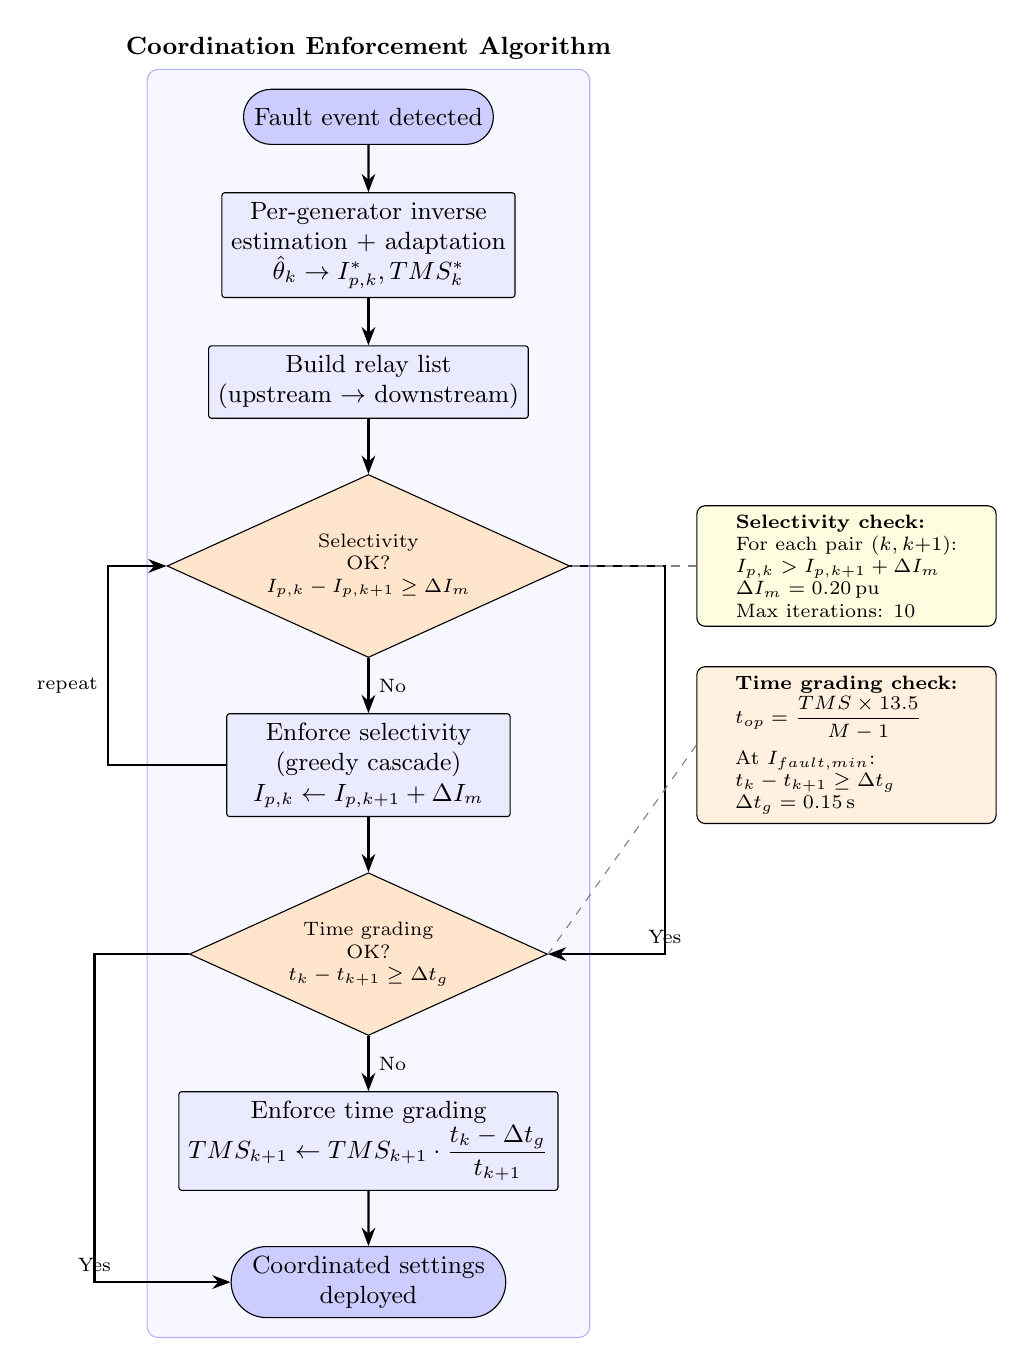
\begin{tikzpicture}[
  font=\small,
  >=Stealth,
  startstop/.style={draw,rounded rectangle,minimum width=2.8cm,minimum height=0.7cm,
                    fill=blue!20,align=center},
  process/.style  ={draw,rectangle,minimum width=3.6cm,minimum height=0.75cm,
                    fill=blue!8,align=center,rounded corners=1pt},
  decision/.style ={draw,diamond,aspect=2.2,minimum height=0.9cm,
                    fill=orange!20,align=center,font=\scriptsize},
  io/.style       ={draw,trapezium,trapezium left angle=75,trapezium right angle=105,
                    minimum width=3.2cm,minimum height=0.7cm,
                    fill=green!12,align=center},
  arrow/.style    ={->,thick},
  ynode/.style    ={font=\scriptsize,pos=0.5},
]

%% ======================================================
%% Layout: two columns
%% Left = Selectivity enforcement, Right = Time grading
%% ======================================================

% --- Selectivity column (left, x=0) ---
\node[startstop] (start) at (0,0) {Fault event detected};
\node[process,below=0.6cm of start]   (estim) {Per-generator inverse\\estimation + adaptation\\$\hat\theta_k \to I_{p,k}^*, TMS_k^*$};
\node[process,below=0.6cm of estim]   (build) {Build relay list\\(upstream $\to$ downstream)};
\node[decision,below=0.7cm of build]  (chksel) {Selectivity\\OK?\\$I_{p,k}-I_{p,k+1}\geq\Delta I_m$};
\node[process,below=0.7cm of chksel]  (enfsel) {Enforce selectivity\\(greedy cascade)\\$I_{p,k}\leftarrow I_{p,k+1}+\Delta I_m$};
\node[decision,below=0.7cm of enfsel] (chktg)  {Time grading\\OK?\\$t_k-t_{k+1}\geq\Delta t_g$};
\node[process,below=0.7cm of chktg]   (enftg)  {Enforce time grading\\$TMS_{k+1}\leftarrow TMS_{k+1}\cdot\dfrac{t_k-\Delta t_g}{t_{k+1}}$};
\node[startstop,below=0.7cm of enftg] (done)   {Coordinated settings\\deployed};

%% --- Arrows (left column) ---
\draw[arrow] (start)   -- (estim);
\draw[arrow] (estim)   -- (build);
\draw[arrow] (build)   -- (chksel);
\draw[arrow] (chksel)  -- node[right,ynode]{No} (enfsel);
\draw[arrow] (chksel.east) -- ++(1.2,0) |- node[above,font=\scriptsize]{Yes}
             (chktg.east);
\draw[arrow] (enfsel)  -- (chktg);
\draw[arrow] (chktg)   -- node[right,ynode]{No} (enftg);
\draw[arrow] (chktg.west) -- ++(-1.2,0) |- node[above,font=\scriptsize]{Yes}
             (done.west);
\draw[arrow] (enftg)   -- (done);

%% --- Repeat loop on selectivity ---
\draw[arrow] (enfsel.west) -- ++(-1.5,0) |- node[pos=0.2,left,font=\scriptsize]
             {repeat} (chksel.west);

%% ======================================================
%%  Right annotation panel
%% ======================================================
\node[draw,fill=yellow!12,rounded corners=3pt,
      right=1.6cm of chksel,align=left,font=\scriptsize,
      minimum width=3.8cm] (note1)
      {\textbf{Selectivity check:}\\
       For each pair $(k, k{+}1)$:\\
       $I_{p,k} > I_{p,k+1} + \Delta I_m$\\
       $\Delta I_m = 0.20\,\text{pu}$\\
       Max iterations: 10};

\node[draw,fill=orange!12,rounded corners=3pt,
      below=0.5cm of note1,align=left,font=\scriptsize,
      minimum width=3.8cm] (note2)
      {\textbf{Time grading check:}\\
       $t_{op} = \dfrac{TMS \times 13.5}{M-1}$\\[3pt]
       At $I_{fault,min}$:\\
       $t_k - t_{k+1} \geq \Delta t_g$\\
       $\Delta t_g = 0.15\,\text{s}$};

\draw[dashed,gray] (note1.west) -- (chksel.east);
\draw[dashed,gray] (note2.west) -- (chktg.east);

\begin{scope}[on background layer]
  \node[draw=blue!30,fill=blue!3,rounded corners=4pt,
        fit=(start)(estim)(build)(chksel)(enfsel)(chktg)(enftg)(done),
        inner sep=7pt,label=above:\textbf{Coordination Enforcement Algorithm}] {};
\end{scope}

\end{tikzpicture}
\end{document}
